
\documentclass{article}

\usepackage{fullpage,latexsym,picinpar,amsmath,amsfonts,graphicx}

           

%%%%%%%%%%%%%%%%%%%%%%%%%%%%%%%%%%%%%%%%%%%%%%%%%%%%%%%%%%%%%%%%%%%%%%%%%%%%%%%%%%%
%%%%%%%%%%%  LETTERS 
%%%%%%%%%%%%%%%%%%%%%%%%%%%%%%%%%%%%%%%%%%%%%%%%%%%%%%%%%%%%%%%%%%%%%%%%%%%%%%%%%%%

\newcommand{\barx}{{\bar x}}
\newcommand{\bary}{{\bar y}}
\newcommand{\barz}{{\bar z}}
\newcommand{\bart}{{\bar t}}

\newcommand{\bfP}{{\bf{P}}}

%%%%%%%%%%%%%%%%%%%%%%%%%%%%%%%%%%%%%%%%%%%%%%%%%%%%%%%%%%%%%%%%%%%%%%%%%%%%%%%%%%%
%%%%%%%%%%%%%%%%%%%%%%%%%%%%%%%%%%%%%%%%%%%%%%%%%%%%%%%%%%%%%%%%%%%%%%%%%%%%%%%%%%%
                                                                                
\newcommand{\parend}[1]{{\left( #1  \right) }}
\newcommand{\spparend}[1]{{\left(\, #1  \,\right) }}
\newcommand{\angled}[1]{{\left\langle #1  \right\rangle }}
\newcommand{\brackd}[1]{{\left[ #1  \right] }}
\newcommand{\spbrackd}[1]{{\left[\, #1  \,\right] }}
\newcommand{\braced}[1]{{\left\{ #1  \right\} }}
\newcommand{\leftbraced}[1]{{\left\{ #1  \right. }}
\newcommand{\floor}[1]{{\left\lfloor #1\right\rfloor}}
\newcommand{\ceiling}[1]{{\left\lceil #1\right\rceil}}
\newcommand{\barred}[1]{{\left|#1\right|}}
\newcommand{\doublebarred}[1]{{\left|\left|#1\right|\right|}}
\newcommand{\spaced}[1]{{\, #1\, }}
\newcommand{\suchthat}{{\spaced{|}}}
\newcommand{\numof}{{\sharp}}
\newcommand{\assign}{{\,\leftarrow\,}}
\newcommand{\myaccept}{{\mbox{\tiny accept}}}
\newcommand{\myreject}{{\mbox{\tiny reject}}}
\newcommand{\blanksymbol}{{\sqcup}}
                                                                                                                         
\newcommand{\veps}{{\varepsilon}}
\newcommand{\Sigmastar}{{\Sigma^\ast}}
                           
\newcommand{\half}{\mbox{$\frac{1}{2}$}}    
\newcommand{\threehalfs}{\mbox{$\frac{3}{2}$}}   
\newcommand{\domino}[2]{\left[\frac{#1}{#2}\right]}  

%%%%%%%%%%%% complexity classes

\newcommand{\PP}{\mathbb{P}}
\newcommand{\NP}{\mathbb{NP}}
\newcommand{\PSPACE}{\mathbb{PSPACE}}
\newcommand{\coNP}{\textrm{co}\mathbb{NP}}
\newcommand{\DLOG}{\mathbb{L}}
\newcommand{\NLOG}{\mathbb{NL}}
\newcommand{\NL}{\mathbb{NL}}

%%%%%%%%%%% decision problems

\newcommand{\PCP}{\sc{PCP}}
\newcommand{\Path}{\sc{Path}}
\newcommand{\GenGeo}{\sc{Generalized Geography}}

\newcommand{\malytm}{{\mbox{\tiny TM}}}
\newcommand{\malycfg}{{\mbox{\tiny CFG}}}
\newcommand{\Atm}{\mbox{\rm A}_\malytm}
\newcommand{\complAtm}{{\overline{\mbox{\rm A}}}_\malytm}
\newcommand{\AllCFG}{{\mbox{\sc All}}_\malycfg}
\newcommand{\complAllCFG}{{\overline{\mbox{\sc All}}}_\malycfg}
\newcommand{\complL}{{\bar L}}
\newcommand{\TQBF}{\mbox{\sc TQBF}}
\newcommand{\SAT}{\mbox{\sc SAT}}

%%%%%%%%%%%%%%%%%%%%%%%%%%%%%%%%%%%%%%%%%%%%%%%%%%%%%%%%%%%%%%%%%%%%%%%%%%%%%%%%%%%
%%%%%%%%%%%%%%% for homeworks
%%%%%%%%%%%%%%%%%%%%%%%%%%%%%%%%%%%%%%%%%%%%%%%%%%%%%%%%%%%%%%%%%%%%%%%%%%%%%%%%%%%

\newcommand{\student}[2]{%
{\noindent\Large{ \emph{#1} SID {#2} } \hfill} \vskip 0.1in}

\newcommand{\assignment}[1]{\medskip\centerline{\large\bf CS 111 ASSIGNMENT {#1}}}

\newcommand{\duedate}[1]{{\centerline{due {#1}\medskip}}}     

\newcounter{problemnumber}                                                                                 

\newenvironment{problem}{{\vskip 0.1in \noindent
              \bf Problem~\addtocounter{problemnumber}{1}\arabic{problemnumber}:}}{}

\newcounter{solutionnumber}

\newenvironment{solution}{{\vskip 0.1in \noindent
             \bf Solution~\addtocounter{solutionnumber}{1}\arabic{solutionnumber}:}}
				{\ \newline\smallskip\lineacross\smallskip}

\newcommand{\lineacross}{\noindent\mbox{}\hrulefill\mbox{}}

\newcommand{\decproblem}[3]{%
\medskip
\noindent
\begin{list}{\hfill}{\setlength{\labelsep}{0in}
                       \setlength{\topsep}{0in}
                       \setlength{\partopsep}{0in}
                       \setlength{\leftmargin}{0in}
                       \setlength{\listparindent}{0in}
                       \setlength{\labelwidth}{0.5in}
                       \setlength{\itemindent}{0in}
                       \setlength{\itemsep}{0in}
                     }
\item{{{\sc{#1}}:}}
                \begin{list}{\hfill}{\setlength{\labelsep}{0.1in}
                       \setlength{\topsep}{0in}
                       \setlength{\partopsep}{0in}
                       \setlength{\leftmargin}{0.5in}
                       \setlength{\labelwidth}{0.5in}
                       \setlength{\listparindent}{0in}
                       \setlength{\itemindent}{0in}
                       \setlength{\itemsep}{0in}
                       }
                \item{{\em Instance:\ }}{#2}
                \item{{\em Query:\ }}{#3}
                \end{list}
\end{list}
\medskip
}

%%%%%%%%%%%%%%%%%%%%%%%%%%%%%%%%%%%%%%%%%%%%%%%%%%%%%%%%%%%%%%%%%%%%%%%%%%%%%%%%%%%
%%%%%%%%%%%%% for quizzes
%%%%%%%%%%%%%%%%%%%%%%%%%%%%%%%%%%%%%%%%%%%%%%%%%%%%%%%%%%%%%%%%%%%%%%%%%%%%%%%%%%%

\newcommand{\quizheader}{ {\large NAME: \hskip 3in SID:\hfill}
                                \newline\lineacross \medskip }


%%%%%%%%%%%%%%%%%%%%%%%%%%%%%%%%%%%%%%%%%%%%%%%%%%%%%%%%%%%%%%%%%%%%%%%%%%%%%%%%%%%
%%%%%%%%%%%%% for final
%%%%%%%%%%%%%%%%%%%%%%%%%%%%%%%%%%%%%%%%%%%%%%%%%%%%%%%%%%%%%%%%%%%%%%%%%%%%%%%%%%%

\newcommand{\namespace}{\noindent{\Large NAME: \hfill SID:\hskip 1.5in\ }\\\medskip\noindent\mbox{}\hrulefill\mbox{}}




\newcommand{\hwduedate}{{8AM, Tuesday, November 22}}

\begin{document}
\student{Robert Martinez}{861238333}

\centerline{\large \bf CS/MATH111 ASSIGNMENT 4}
\centerline{due {\hwduedate}}

\vskip 0.2in
\noindent{\bf Individual assignment:} Problems 1 and 2.

\noindent{\bf Group assignment:} Problems 1,2 and 3.

\vskip 0.15in

%%%%%%%%%%%%%%%%%%%%%%%%%%%%


\begin{problem}
Give the asymptotic value (using the $\Theta$-notation)
for the number of letters that will be printed by the algorithms below.
In each algorithm the argument $n$ is a positive integer.
Your solution needs to consist of an appropriate recurrence 
equation and its solution, including a justification for both. 

\bigskip
\noindent
(a)\ \ 
\begin{minipage}[t]{3in}
\begin{tabbing}
aaa \= aaa \= aaa \= aaa \=  \kill
\textbf{Algorithm} \textsc{PrintAs} $(n: \mbox{\bf integer})$ \\
          \> \textbf{if} $n < 3$ \\
          \>\>  print(``A") \\
          \>\textbf{else} \\
          	\>\> \textsc{PrintAs}$(\ceiling{n/3})$\\
      		\>\> \textbf{for} $i \leftarrow 1$ \textbf{to} $9$ \textbf{do} print(``A")
\end{tabbing}
\end{minipage}

\bigskip
\noindent
(b)\ \
\begin{minipage}[t]{3in}
\begin{tabbing}
aaa \= aaa \= aaa \= aaa \=  \kill
\textbf{Algorithm} \textsc{PrintBs} $(n: \mbox{\bf integer})$ \\
          \> \textbf{if} $n < 3$ \\
          \>\>  print(``B") \\
          \>\textbf{else} \\
          \>\>  \textsc{PrintBs}$(\floor{n/3})$\\
         \>\>  \textsc{PrintBs}$(\ceiling{n/3})$\\
      \>\> \textbf{for} $i \leftarrow 1$ \textbf{to} $9n$ \textbf{do} print(``B")
\end{tabbing}
\end{minipage}

\bigskip
\noindent
(c)\ \ 
\begin{minipage}[t]{3in}
\begin{tabbing}
aaa \= aaa \= aaa \= aaa \=  \kill
\textbf{Algorithm} \textsc{PrintCs} $(n: \mbox{\bf integer})$ \\
          \> \textbf{if} $n < 3$ \\
          \>\>  print(``C") \\
          \>\textbf{else} \\
         	\>\>  \textsc{PrintCs}$(\ceiling{n/3})$\\
			\>\>  \textsc{PrintCs}$(\ceiling{n/3})$\\
			\>\>  \textsc{PrintCs}$(\ceiling{n/3})$\\
      	  	\>\> \textbf{for} $i \leftarrow 1$ \textbf{to} $9n$ \textbf{do} print(``C")
\end{tabbing}
\end{minipage}

\bigskip
\noindent
(d)\ \ 
\begin{minipage}[t]{3in}
\begin{tabbing}
aaa \= aaa \= aaa \= aaa \=  \kill
\textbf{Algorithm} \textsc{PrintDs} $(n: \mbox{\bf integer})$ \\
          \> \textbf{if} $n < 3$ \\
          \>\>  print(``D") \\
          \>\textbf{else} \\
         		\>\>  \textbf{for} $j \leftarrow 1$ \textbf{to} $4$ \textbf{do} \textsc{PrintDs}$(\ceiling{n/3})$\\
				\>\> \textbf{for} $i \leftarrow 1$ \textbf{to} $9 n$ \textbf{do} print(``D")
\end{tabbing}
\end{minipage}


\bigskip
\noindent
(e)\ \ 
\begin{minipage}[t]{3in}
\begin{tabbing}
aaa \= aaa \= aaa \= aaa \=  \kill
\textbf{Algorithm} \textsc{PrintEs} $(n: \mbox{\bf integer})$ \\
          \> \textbf{if} $n < 3$ \\
          \>\>  print(``E") \\
          \>\textbf{else} \\
         		\>\>  \textbf{for} $j \leftarrow 1$ \textbf{to} $4$ \textbf{do} \textsc{PrintEs}$(\ceiling{n/3})$\\
  				\>\> \textbf{for} $i \leftarrow 1$ \textbf{to} $9 n^2$ \textbf{do} print(``E")
\end{tabbing}
\end{minipage}



\end{problem}
\vfill
\eject
%%%%%%%%%%%%%%%%%%%%% Solution 1 %%%%%%%%%%%%%%%%%%%%%%%%
\begin{solution}
\newline

a)
\newline
  
Because ther is the statement: if $n < 3$ followed by a print("A") we know that for $n \ge 3$
\newline

The Recurrence Equation:
\newline

$A(n) = A(n/3)$ +9
\newline

Solving the recurrance equation:
\newline

Using the Master Theorem where $a=1$, $b=3$, $c=9$, $d=0$ we see that:
\newline

$1 = 3^0$
\newline

$1=1$
\newline

By the Master Theorem:
\newline

$A(n) = \Theta(logn)$
\newline

b)
\newline

for $n > 3$:
\newline

The recurrence equation is:
\newline

$B(n) = 2B(n/3) +9n$
\newline

The $2B(n/3)$ comes from the two recurrance calls, and the 9n comes from the parameters in the for loop.
\newline

Solving the recurrence equation using the Master Theorem where $a=2$, $b=3$, $c=9$, $d=1$  we see that:
\newline

$a>b^d$
\newline

$2>3^1$
\newline

By the Master Theorem:
\newline

for $a<b^d$; $f_n = \Theta(n^d)$
\newline

$B(n) = \Theta(n^1)$
\newline

$B(n) = \Theta(n)$
\newline

c)
\newline

for $n > 3$:
\newline

The recurrence equation is:
\newline

$C(n) = 3C(n/3) + 9n$
\newline

This is because there are 3 recursive calls and a forloop that prints("C") 9n times.
\newline
\indent Solving the recurrnace equation using the Master Theorem where: $a=2$, $b=3$, $c=9$, $d=1$  we see that:
\newline

$a = b^d$
\newline

$3 = 3^1$
\newline

By the Master Theorem:
\newline

for $a=b^d$; $f_n = \Theta(n^d logn)$
\newline

So:
\newline

$C(n) = \Theta(n^1 logn)$
\newline

$C(n) = \Theta(nlogn)$
\newline

d)
\newline

for $n > 3$:
\newline

The recurrence equation is:
\newline

$D(n) = 4D(n/3) + 9n$
\newline

This is because there are 4 recursive calls and a forloop that prints("D") 9n times.
\newline

\indent Solving the recurrnace equation using the Master Theorem where: $a=4$, $b=3$, $c=9$, $d=1$  we see that:
\newline

$4 > 3^1$
\newline

$a > b^d$
\newline

By the Master Theorem:
\newline

for $a > b^d$; $f_n = \Theta(n^{log_b a})$
\newline

So:
\newline

$D(n) = \Theta(n^{log_3 4})$
\newline

e)
\newline

for $n > 3$:
\newline

The recurrence equation is:
\newline

$E(n) = 4E(n/3) + 9n^2$
\newline

This is because there are 4 recursive calls and a forloop that prints("D") $9n^2$ times.
\newline

\indent Solving the recurrnace equation using the Master Theorem where: $a=4$, $b=3$, $c=9$, $d=2$  we see that:
\newline

$4<3^2$
\newline

$a<b^d$
\newline

By the Master Theorem:
\newline

for $a < b^d$; $f_n = \Theta(n^d)$
\newline

So:
\newline

$E(n) = \Theta(n^2)$
\newline



\end{solution}
%%%%%%%%%%%%%%%%%%%%%%%%%%%% End Solution 2 %%%%%%%%%%%%%5

\begin{problem}
For each integer $n \ge 1$ we define a tree $T_n$, recursively, as follows. $T_1$ consists of only
a single node. For $n \ge 2$, $T_n$ is obtained from four copies of $T_{\floor{n/2}}$ and three 
additional nodes, by connecting them as follows:
%
\begin{center}
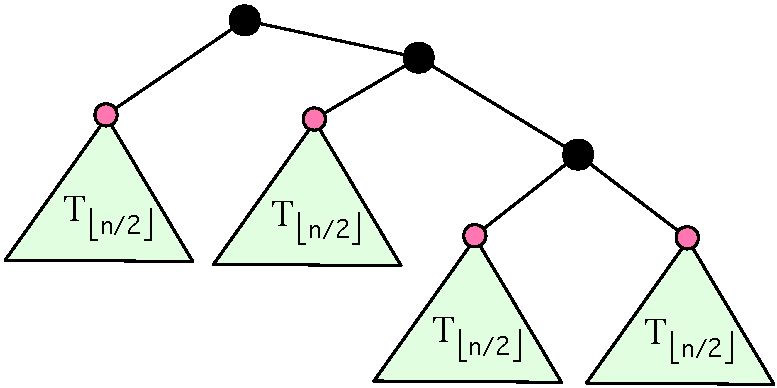
\includegraphics[width=2.5in]{treeforhw4.pdf}
\end{center}
%

\smallskip
\noindent
Let $s(n)$ be the number of nodes in $T_n$. 

\smallskip
\noindent
(a) Give a recurrence equation for $s(n)$ and justify it.

\smallskip
\noindent
(b) Determine the exact values of $s(n)$ for $n = 1,2,3,4,5,6,7,8,9$. (Use the table formatting, as show at the end of the homework.)

\smallskip
\noindent
(c) Draw $T_5$. (You can use a drawing software or draw it by hand, and include a pdf file in the latex source.)

\smallskip
\noindent
(d) Give the asymptotic formula for $s(n)$, by solving the recurrence from part~(a). Justify your solution.
\end{problem}

%%%%%%%%%%%%%%%%%%%%%%%%%%% Solution 2 %%%%%%%%%%%%%%%%%%%%%%%%%%%%

\begin{solution}

\newline
a)
\newline

The inital condition is:
\newline

for $n \ge 1$:
\newline

$s(n) = 4s_{\floor{n/2}}$
\newline

This is the recurrance eqaution because there are 4 recursive calls to $T_{\floor{n/2}}$ (which is rounded down) plus an additional 3 nodes.
\newline





b)
\newline

\begin{tabular}{|r|p{0.15in}|p{0.15in}|p{0.15in}|p{0.15in}|p{0.15in}|p{0.15in}|p{0.15in}|p{0.15in}|p{0.15in}|} \hline
$n$     & 1 & 2 & 3 & 4 & 5 & 6 & 7 & 8 & 9  
\\ \hline
$s(n)$    & 1 & 7 & 7 & 31 & 31 & 31 & 31 & 127 & 127 
\\ \hline
\end{tabular}
\newline

\newline
c)
\newline

This is T_5:
\begin{center}
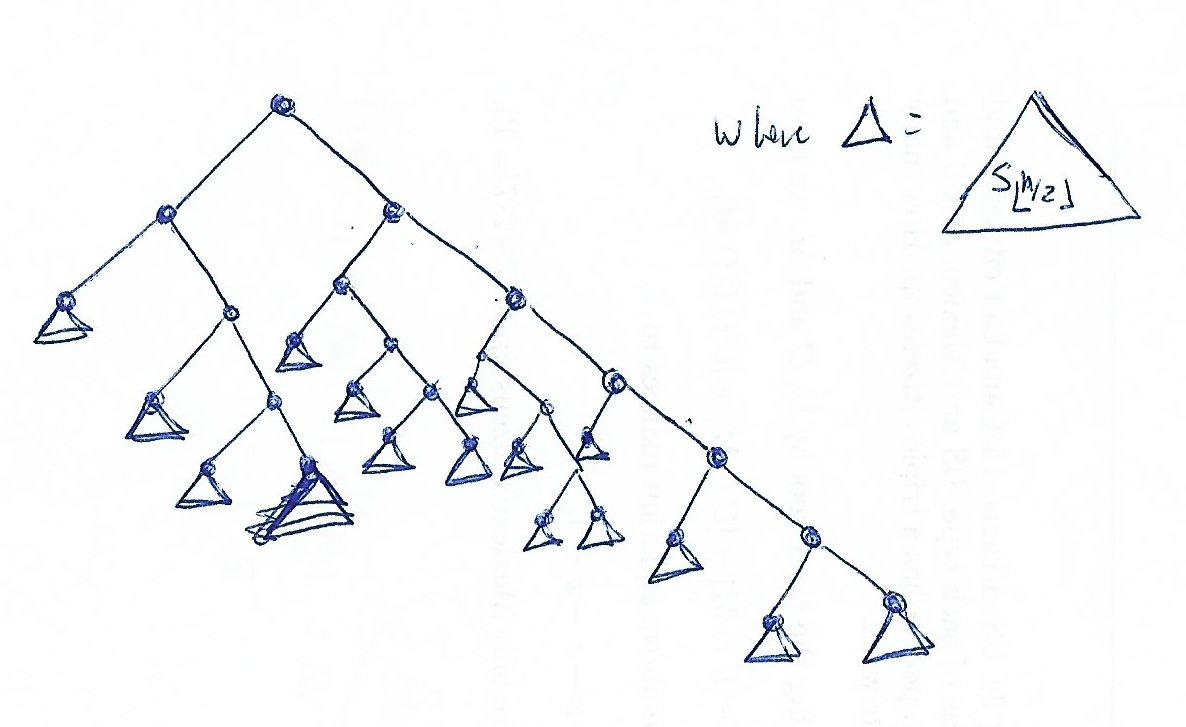
\includegraphics[width=2.5in]{tree.jpg}
\end{center}
\newline

d)
\newline

Given the recurance equation $s(n) = 4s_{\floor{n/2}} +3$
\newline

Using the Master Theorem where $a=4$, $b=3$, $c=3$, and $d=0$:
\newline

$a>b^d$
\newline

$4>2^0$
\newline

By the Master theorem when $a>b^d$, $\Theta(n^{log_b a})$
\newline

$s(n) = \Theta(n^{log_2 4})$
\newline

So the asymptotic formula for the equation is:
\newline

$s(n) = \Theta(n^2)$
\newline






\end{solution}
%%%%%%%%%%%%%%%%%%%%%%%%%%%%

\begin{problem}
RockCyc is a mountain bicycle that is available with three upgrade options:
for the fork, brakes, or wheels. 105 customers bought a RockCyc bike. Among them:
%
\begin{itemize}
	\item 45 upgraded fork
	\item 36 upgraded brakes
	\item 25 upgraded wheels
	\item 17 upgraded fork and brakes
	\item 13 upgraded fork and wheels
	\item 10 upgraded brakes and wheels
	\item 4 upgraded all three components
\end{itemize}
%
(To clarify, these categories are not exclusive. For example, the set of 45 customers that upgraded
the fork includes those that upgraded the fork and the brakes.)

Use the inclusion-exclusion principle to determine how many customers bought the basic model
of RockCyc, without any upgrades.
Show your work.
\end{problem}

%%%%%%%%%%%%%%%%%%%%%%%%%%%%


\vskip 0.15in
\paragraph{Submission.}
To submit the homework, you need to upload the pdf file into ilearn by {\hwduedate},
and turn-in a paper copy in class.

\bigskip
\noindent
\hrule

\bigskip

\noindent
Here is how you can format the table for the solution of Problem~2b:


\bigskip
\noindent
\begin{tabular}{|r|p{0.15in}|p{0.15in}|p{0.15in}|p{0.15in}|p{0.15in}|p{0.15in}|p{0.15in}|p{0.15in}|p{0.15in}|} \hline
$n$ 		& 1 & 2 & 3 & 4 & 5 & 6 & 7 & 8 & 9  
\\ \hline
$s(n)$		& a & b & c & d & e & f & g & h & i 
\\ \hline
\end{tabular}

\end{document}

